\chapter{Metodologia}
\label{chap:metodologia}


% ==============================================================================
% METODOLOGIA — Seleção da coorte e pré-processamento dos dados
% Baseado em processamento_gpu.py (classe PassandoDadosClassificacao)
%
% Valores conferidos no código em 06/10/2026:
%   filtro      Butterworth ordem 3, 0,5-40 Hz, fase nula (sosfiltfilt)
%   escala      percentil 99 do valor absoluto, por derivação
%   corte       +-5 após a normalização
%   margem      5 min no início e no fim do registro
%   validação   25% do treino de cada partição (frac_val = 0.25)
% ==============================================================================

\section{População de estudo}
\label{sec:met-coorte}
\label{sec:intro-dados}

\subsection{Base de dados}
\label{subsec:met-base}

Os dados deste trabalho provêm da base \gls{MUSIC}, disponibilizada
publicamente no PhysioNet \cite{martinyebra2025music, martinyebra2024music}.
A base reúne 992 pacientes com insuficiência cardíaca crônica sintomática
(classes II e III da \textit{New York Heart Association}), recrutados entre
abril de 2003 e dezembro de 2004 em oito hospitais universitários da Espanha
e acompanhados por uma mediana de 44 meses. Para 936 deles há um registro de
Holter de 24~horas, com três derivações ortogonais (X, Y e Z) amostradas a
200\,Hz, e as causas de óbito foram adjudicadas segundo definições
explícitas, que separam a \gls{MSC} do óbito por falência de bomba. Além do
Holter, a base fornece, para cada paciente, variáveis clínicas e resultados
de exames realizados na entrada do estudo, descritos na
\autoref{subsec:met-clinicas}.

Três características tornam a MUSIC adequada ao problema estudado. Primeiro,
trata-se de uma população em que a \gls{MSC} é um desfecho frequente e
clinicamente relevante, e não de uma amostra da população geral, na qual o
evento seria raro demais para o aprendizado. Segundo, o Holter de 24~horas
oferece uma observação longa do \gls{ECG}, que capta variações ao longo do
dia inacessíveis a um traçado de repouso de poucos segundos. Terceiro, a
adjudicação do mecanismo de óbito permite isolar a morte de origem elétrica,
que é o objeto deste trabalho.

\begin{figure}[h!]
	\captionsetup{width=14cm}
	\Caption{\label{fig:fluxograma-coorte} Fluxograma de seleção da coorte}
	\UFCfig{}{
		\makebox[\linewidth]{\begin{tikzpicture}[
				x=1cm, y=1cm,
				etapa/.style={draw, rounded corners=2pt, fill=gray!8, align=center,
						text width=5.6cm, minimum height=1.0cm, font=\small},
				exclui/.style={draw, rounded corners=2pt, fill=red!6, align=left,
						text width=6.6cm, font=\small},
				final/.style={etapa, fill=green!8, line width=0.8pt},
				seta/.style={-{Stealth[length=2.2mm]}, thick},
			]
			\node[etapa] (n0) at (0, 0)     {Pacientes na base MUSIC\\\textbf{992}};
			\node[etapa] (n1) at (0, -2.3)  {Em ritmo sinusal\\\textbf{710}};
			\node[etapa] (n2) at (0, -4.9)  {Óbito por MSC ou vivo\\\textbf{608}};
			\node[etapa] (n3) at (0, -7.5)  {Casos + controles\\\textbf{587}};
			\node[final] (n4) at (0, -10.1) {Coorte final: \textbf{517}\\55 casos (MSC) e 462 controles};
			\foreach \a/\b in {n0/n1, n1/n2, n2/n3, n3/n4} \draw[seta] (\a) -- (\b);
			\node[exclui] (e1) at (6.9, -1.15) {\textbf{Critério 1} --- excluídos 282:\\ritmo não sinusal no Holter\\(fibrilação/\textit{flutter} atrial, marcapasso)};
			\node[exclui] (e2) at (6.9, -3.6)  {\textbf{Critério 2} --- excluídos 102:\\35 óbitos de causa não cardíaca\\67 óbitos por falência de bomba};
			\node[exclui] (e3) at (6.9, -6.2)  {\textbf{Critério 3} --- excluídos 21:\\\emph{apenas vivos} com seguimento inferior a\\4 anos (1\,460 dias); não se aplica aos\\óbitos por MSC};
			\node[exclui] (e4) at (6.9, -8.8)  {\textbf{Sinal} --- excluídos 70:\\47 sem registro de Holter\\23 sem as três derivações (X, Y e Z)};
			\draw[seta] (0, -1.15) -- (e1.west);
			\draw[seta] (0, -3.6)  -- (e2.west);
			\draw[seta] (0, -6.2)  -- (e3.west);
			\draw[seta] (0, -8.8)  -- (e4.west);
		\end{tikzpicture}}
	}{
		\Fonte{elaborado pelo autor (2026).}
	}
\end{figure}

\FloatBarrier

\subsection{Definição da população e critérios de seleção}
\label{subsec:met-criterios}

O problema foi formulado como uma classificação binária no nível do
paciente: a partir do Holter, distinguir quem veio a óbito por \gls{MSC} de
quem sobreviveu ao período de acompanhamento de quatro anos. Essa
formulação exige que o rótulo de cada paciente seja inequívoco, e os
critérios de seleção decorrem dessa exigência. A partir dos 992 pacientes da
base, a população foi definida pelos três critérios a seguir, resumidos na
\autoref{fig:fluxograma-coorte} e na \autoref{tab:fluxo-music}.

\textbf{Critério 1: ritmo sinusal durante o Holter.} Foram excluídos os
pacientes cujo registro foi anotado com ritmo diferente do sinusal (282
pacientes, com fibrilação atrial permanente, \textit{flutter} atrial ou
ritmo de marcapasso). Na fibrilação atrial não há onda P organizada e os
intervalos entre batimentos são irregulares por definição, de modo que as
medidas de variabilidade da frequência cardíaca e de morfologia perdem o
significado fisiológico que têm em ritmo sinusal; o ritmo de marcapasso,
por sua vez, não reflete a atividade elétrica espontânea do coração. Além
disso, o próprio ritmo está associado ao risco: incluí-lo permitiria que um
modelo aprendesse a reconhecer a arritmia atrial, e não marcadores de
vulnerabilidade elétrica ventricular.

\textbf{Critério 2: classe 0 (sobreviventes) e classe 3 (morte súbita
cardíaca).} Foram mantidos apenas os pacientes vivos ao fim do
acompanhamento (classe 0 da variável de causa de óbito), que formam o grupo
de controles, e os pacientes com óbito adjudicado como \gls{MSC} (classe 3),
que formam o grupo de casos. Foram excluídos os óbitos por falência de bomba
(67 pacientes), cujo mecanismo é mecânico e progressivo, e os óbitos de
causa não cardíaca (35 pacientes). Incluir a falência de bomba entre os
casos ensinaria o modelo a reconhecer a gravidade da insuficiência cardíaca
em geral, e não o risco específico de morte súbita; incluí-la entre os
controles colocaria do lado ``sem evento'' pacientes que também morreram de
causa cardíaca.

\textbf{Critério 3: exclusão dos sobreviventes que deixaram o acompanhamento
antes de quatro anos.} Foram excluídos os pacientes da classe 0 com
seguimento inferior a 1\,460~dias (21 pacientes). Um sobrevivente observado
por menos de quatro anos pode ter sofrido o evento depois de deixar o
estudo, e rotulá-lo como controle introduziria erro no rótulo. O critério
não se aplica aos casos, cujo desfecho já foi observado.

Por fim, exigiu-se a presença das três derivações no registro de Holter:
foram excluídos 47 pacientes sem registro disponível e 23 cujo registro não
continha a derivação Z. A população final compreendeu 517 pacientes, dos
quais 55 casos de \gls{MSC} e 462 controles, com prevalência de 10,6\,\%.







\begin{table}[htbp]
	\centering
	\caption{Fluxo de seleção da base MUSIC e disponibilidade dos registros de Holter.}
	\label{tab:fluxo-music}
	\begin{tabular}{lr}
		\hline
		\textbf{Etapa}                                & \textbf{N} \\
		\hline
		Registros de Holter na base (total)           & 936        \\
		Pacientes na base MUSIC                       & 992        \\
		\quad Excluídos: ritmo não sinusal            & 282        \\
		Em ritmo sinusal                              & 710        \\
		\quad Excluídos por desfecho ambíguo          & 123        \\
		\qquad Morte não cardíaca (código 1)          & 35         \\
		\qquad Falência de bomba (códigos 6 e 7)      & 67         \\
		\qquad Vivos com seguimento inferior a 4 anos & 21         \\
		Casos + controles                             & 587        \\
		\quad Sem registro de Holter                  & 47         \\
		\quad Registro sem derivação Z                & 23         \\
		Analisados                                    & 517        \\
		\quad Casos (MSC; prevalência de 10,6\%)      & 55         \\
		\quad Controles                               & 462        \\
		\hline
	\end{tabular}
\end{table}

Os critérios têm um custo. A restrição ao ritmo sinusal e a exclusão dos
desfechos ambíguos reduzem a população a pouco mais da metade da base, e os
resultados se aplicam a pacientes com insuficiência cardíaca em ritmo
sinusal, sem poderem ser estendidos, sem nova avaliação, a pacientes com
fibrilação atrial. Optou-se por essa troca porque um rótulo confiável e um
sinal de entrada homogêneo são pré-requisitos para que um resultado,
positivo ou negativo, possa ser interpretado.


\FloatBarrier

\subsection{Variáveis clínicas e exames}
\label{subsec:met-clinicas}

Nos experimentos que combinam o sinal a variáveis clínicas, foram empregadas
seis, de três tipos: a idade, variável numérica de valor inteiro, em anos; a
classe funcional \gls{NYHA}, variável categórica ordinal; e quatro variáveis
binárias, codificadas como 0 (ausente) ou 1 (presente) --- gênero (1 =
masculino), presença de ondas Q de necrose no \gls{ECG} de repouso,
taquicardia ventricular não sustentada (TVNS)\glsadd{TVNS}\glsunset{TVNS} e
taquiarritmia supraventricular paroxística. A idade e a classe \gls{NYHA}
foram padronizadas pela média e pelo desvio-padrão do conjunto de
treinamento de cada partição.

Duas particularidades da coorte merecem registro. A classe funcional \gls{NYHA}
assume apenas os valores II e III, comportando-se, na prática, como variável
binária. A variável de taquiarritmia supraventricular paroxística é
originalmente categórica nominal, com códigos para taquicardia
supraventricular, fibrilação atrial paroxística, \textit{flutter} e outras;
o código de ausência por fibrilação atrial crônica deixa de ocorrer após a
restrição ao ritmo sinusal, e a variável foi tratada como indicadora da
presença de qualquer episódio.



Além dessas seis variáveis, a base fornece os resultados de exames
realizados na entrada do estudo, empregados no Cenário III
(\autoref{sec:met-cenario3}) e agrupados por origem: o ecocardiograma e a
radiografia de tórax (\gls{FEVE}, tamanho do átrio esquerdo, diâmetros
diastólico e sistólico do ventrículo esquerdo, espessuras do septo e da
parede posterior, diâmetro e contratilidade do ventrículo direito e índice
cardiotorácico), todos numéricos de valor real, exceto a contratilidade do
ventrículo direito, binária; o laudo do \gls{ECG} de repouso (intervalos PR
e QT, QT corrigido e duração do QRS, numéricos, e QRS acima de 120\,ms,
hipertrofia ventricular esquerda e distúrbio de condução intraventricular,
binários); as medidas do Holter tabuladas pela equipe do estudo (intervalos
RR mínimo e máximo e sua amplitude, número de extrassístoles ventriculares e
supraventriculares em 24~horas, dupletes, \gls{SDNN}, SDANN, \gls{RMSSD} e
pNN50, numéricos); e o exame laboratorial do Pro-BNP, numérico. As
contagens de extrassístoles e o Pro-BNP, de distribuição muito assimétrica,
foram transformados por $\log(1+x)$.


\section{Pré-processamento do sinal}
\label{sec:met-preprocessamento}

Cada registro de Holter contém três derivações, X, Y e Z, amostradas a
200\,Hz ao longo de cerca de 24~horas. A \autoref{fig:met-ecg-amostra}
mostra, como exemplo, um trecho de 10~segundos de um paciente controle da
coorte, sorteado aleatoriamente, após a filtragem descrita na
\autoref{subsec:met-filtragem}. As três derivações registram os mesmos
batimentos sob ângulos diferentes, o que se reflete na amplitude e na forma
distintas dos complexos QRS e das ondas T em cada uma.

\begin{figure}[h!]
	\captionsetup{width=15cm}
	\Caption{\label{fig:met-ecg-amostra} Trecho de 10 segundos do Holter de um
		paciente controle da coorte, nas derivações X, Y e Z, após o filtro
		passa-faixa de 0,5 a 40\,Hz}
	\UFCfig{}{
		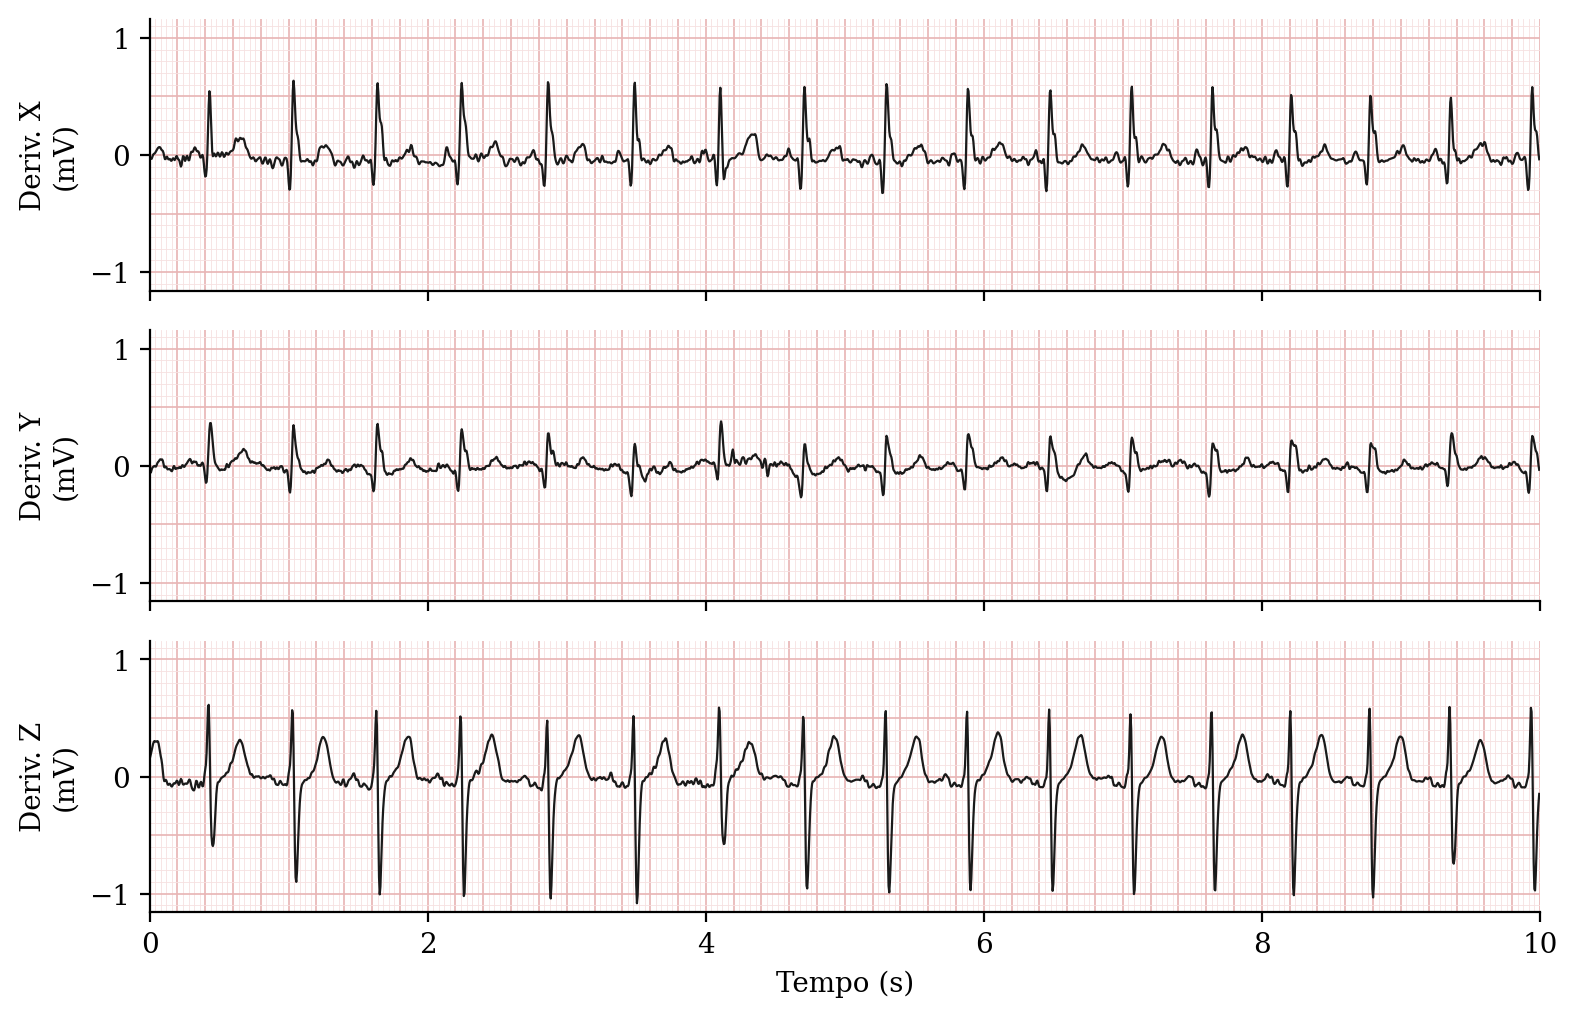
\includegraphics[width=15cm]{figuras/ecg_tres_derivacoes.png}
	}{
		\Fonte{elaborado pelo autor (2026), a partir da base MUSIC. Grade no
			padrão do papel de \gls{ECG}: 0,2\,s e 0,5\,mV nas linhas fortes.}
	}
\end{figure}


\subsection{Extração de janelas}
\label{subsec:met-janelas}

Cada registro foi representado por janelas de 24\,000 amostras, equivalentes
a dois minutos a 200\,Hz. Os cinco minutos iniciais e finais de cada registro
foram descartados, por concentrarem artefatos de calibração do equipamento,
de acomodação do paciente e de retirada dos eletrodos.

As posições das janelas foram definidas de modo distinto no treinamento e na
avaliação. Nas redes residuais e com concatenação, cada uma das 250 janelas de
treinamento por paciente teve sua
posição sorteada a cada época, de forma independente, ao longo do trecho
útil do registro. O procedimento expõe o modelo a recortes diferentes a cada
passagem pelos dados e admite sobreposição entre janelas. Na avaliação, as
100 janelas por paciente foram posicionadas em grade regular, igualmente
espaçadas ao longo do registro, o que torna as métricas reprodutíveis. Nas
redes convolucionais, implementadas posteriormente, a amostragem foi
refinada para 350 janelas de treinamento sem sobreposição e 200 de
avaliação, conforme a \autoref{subsec:met-cnn-experimentos}.

\subsection{Filtragem}
\label{subsec:met-filtragem}

Cada janela foi submetida a filtro passa-faixa de Butterworth de terceira
ordem, com frequências de corte de 0,5 e 40\,Hz, implementado em seções de
segunda ordem e aplicado nos sentidos direto e reverso. A filtragem de fase
nula resultante dobra a ordem efetiva do filtro e preserva a morfologia das
ondas, conforme discutido na \autoref{subsubsec:fund-fase-nula}.

A frequência de corte inferior remove a oscilação de linha de base e o
deslocamento contínuo do sinal, que varia entre pacientes conforme o
posicionamento dos eletrodos. A superior atenua o ruído muscular e elimina a
interferência da rede elétrica de 50\,Hz, situada acima da banda passante. O
valor de 0,5\,Hz encontra-se dentro do limite admitido pela American Heart
Association para filtros digitais de fase nula
\cite{kligfield2007recommendations}.

A filtragem foi aplicada a cada janela individualmente, e não ao registro
completo. A escolha torna o deslocamento de linha de base removido
específico de cada trecho, sem pressupor estabilidade ao longo das 24\,horas.

\subsection{Normalização}
\label{subsec:met-normalizacao}

Após a filtragem, cada derivação foi dividida por uma constante de escala
global, comum a todos os pacientes. A constante corresponde ao percentil 99
do valor absoluto do sinal filtrado, estimado sobre 100 pacientes sorteados
do conjunto de treinamento de cada partição, com cinco janelas de 60\,s por
paciente. As janelas usadas na estimativa passam pelo mesmo filtro aplicado
no treinamento, de modo que a escala corresponde à distribuição efetivamente
apresentada ao modelo.

A estimativa é refeita a cada partição da validação cruzada, utilizando
exclusivamente pacientes do respectivo conjunto de treinamento. Calculá-la
uma única vez sobre a coorte completa introduziria informação dos pacientes
de teste no pré-processamento.

Os valores normalizados foram limitados ao intervalo $[-5, 5]$. Amostras fora
desse intervalo correspondem a amplitudes superiores a cinco vezes a
referência de escala, ocorrência compatível com artefato de movimento e não
com atividade cardíaca.

A separação entre filtragem e normalização é deliberada. A filtragem por
janela remove o deslocamento individual de cada trecho; a escala global
preserva as diferenças de amplitude entre pacientes. A padronização por
janela, alternativa descartada, realizaria as duas operações
simultaneamente e eliminaria a informação de amplitude absoluta.


% ==============================================================================
% CENARIO I — aprendizado profundo sobre o sinal bruto
% ==============================================================================

\section{Cenário I: aprendizado profundo sobre o sinal bruto}
\label{sec:met-cenario1}
\label{sec:met-redes}

No primeiro cenário, redes neurais profundas recebem o sinal do Holter,
apenas filtrado e normalizado conforme a \autoref{sec:met-preprocessamento},
e são treinadas diretamente para prever a \gls{MSC}. Cada rede recebe janelas
do sinal, produz uma probabilidade por janela e é avaliada no nível do
paciente, após a agregação descrita na \autoref{subsec:fund-agregacao}. Os
fundamentos de cada componente foram apresentados no
\autoref{cap:fundamentacao-teorica}; esta seção descreve as arquiteturas
construídas e as escolhas de treinamento efetivamente adotadas.


\subsection{Arquiteturas avaliadas}
\label{subsec:met-arquiteturas}

As arquiteturas foram organizadas em três famílias, avaliadas em ordem
crescente de complexidade, e a rede profunda com variáveis clínicas concatenadas, que
compartilha o mesmo extrator e é avaliada no Cenário III
(\autoref{sec:met-cenario3}). A \autoref{tab:met-arquiteturas} resume cada uma
delas.

\begin{enumerate}
	\item \textbf{Redes convolucionais sem atalhos.} A rede convolucional
	      descrita na \autoref{sec:fund-cnn}, em três variantes de capacidade ---
	      mínima, simples e média --- que diferem apenas no número de blocos e de
	      filtros. É a família de menor capacidade e serve de referência para as
	      demais.

	\item \textbf{Redes residuais.} Adaptações unidimensionais da ResNet
	      \cite{he2016deep}, na linha das redes empregadas para a classificação de
	      \gls{ECG} por \citeonline{hannun2019cardiologist} e
	      \citeonline{ribeiro2020automatic}. Foram avaliadas profundidades de 18, 34
	      e 50 camadas e, para a profundidade de 18 camadas, três larguras, de modo a
	      separar o efeito da profundidade do efeito do número de canais.

	\item \textbf{Rede residual com atenção.} A ResNet-18 seguida de um
	      codificador \textit{Transformer} \cite{vaswani2017attention}, que recebe a
	      sequência de vetores produzida pelo último estágio residual e permite que
	      cada trecho da janela seja relacionado aos demais antes do agrupamento.

\end{enumerate}

\begin{table}[h!]
	\captionsetup{width=15.5cm}
	\Caption{\label{tab:met-arquiteturas} Arquiteturas de redes neurais
		avaliadas sobre o sinal de Holter}
	\IBGEtab{}{
		\begin{tabular}{llrl}
			\toprule
			Família       & Variante                         & \multicolumn{1}{c}{Parâmetros} & Entrada             \\
			\midrule \midrule
			Convolucional & mínima (3 blocos)                & 14\,425                        & 2 min e 10 s        \\
			              & simples (4 blocos)               & 109\,361                       & 2 min e 10 s        \\
			              & média (4 blocos)                 & 418\,145                       & 2 min e 10 s        \\
			\midrule
			Residual      & ResNet-18 mínima                 & 78\,169                        & 5,12 s              \\
			              & ResNet-18 reduzida               & 1\,029\,985                    & 2 min               \\
			              & ResNet-18                        & 3\,976\,385                    & 2 min e 5,12 s      \\
			              & ResNet-34                        & 7\,350\,721                    & 2 min               \\
			              & ResNet-50                        & 16\,479\,937                   & 2 min               \\
			\midrule
			Atenção       & ResNet-18 + \textit{Transformer} & 1\,491\,553                    & 2 min               \\
			\midrule
			Concatenação  & ResNet-18 + variáveis clínicas  & 3\,987\,041                    & 2 min + 6 variáveis \\
			\bottomrule
		\end{tabular}
	}{
		\Fonte{elaborado pelo autor (2026).}
	}
\end{table}

Todas as variantes compartilham o mesmo classificador final --- agrupamento
global por média e máximo, seguido de duas camadas totalmente conectadas com
descarte --- e a mesma saída: um único \textit{logit} por janela, convertido
em probabilidade pela \autoref{eq:logistica}. A diferença entre elas está
apenas no extrator de características, o que permite atribuir as diferenças
de desempenho à arquitetura.


% ==============================================================================

\subsection{Arquitetura da rede convolucional}
\label{subsec:fund-cnn-arquitetura}

A rede convolucional adotada neste trabalho é composta por blocos
sequenciais, seguidos de agrupamento global e de um classificador de duas
camadas. Cada bloco aplica, nesta ordem, convolução, normalização em lote,
ativação \textit{ReLU}, agrupamento máximo com fator quatro e descarte com
probabilidade 0,1. A \autoref{fig:cnn-arquitetura} ilustra o fluxo.

% ---- FIGURA: diagrama da arquitetura ----
\begin{figure}[h!]
	\captionsetup{width=16cm}
	\Caption{\label{fig:cnn-arquitetura} Arquitetura da rede convolucional
		unidimensional}
	\UFCfig{}{
		\fbox{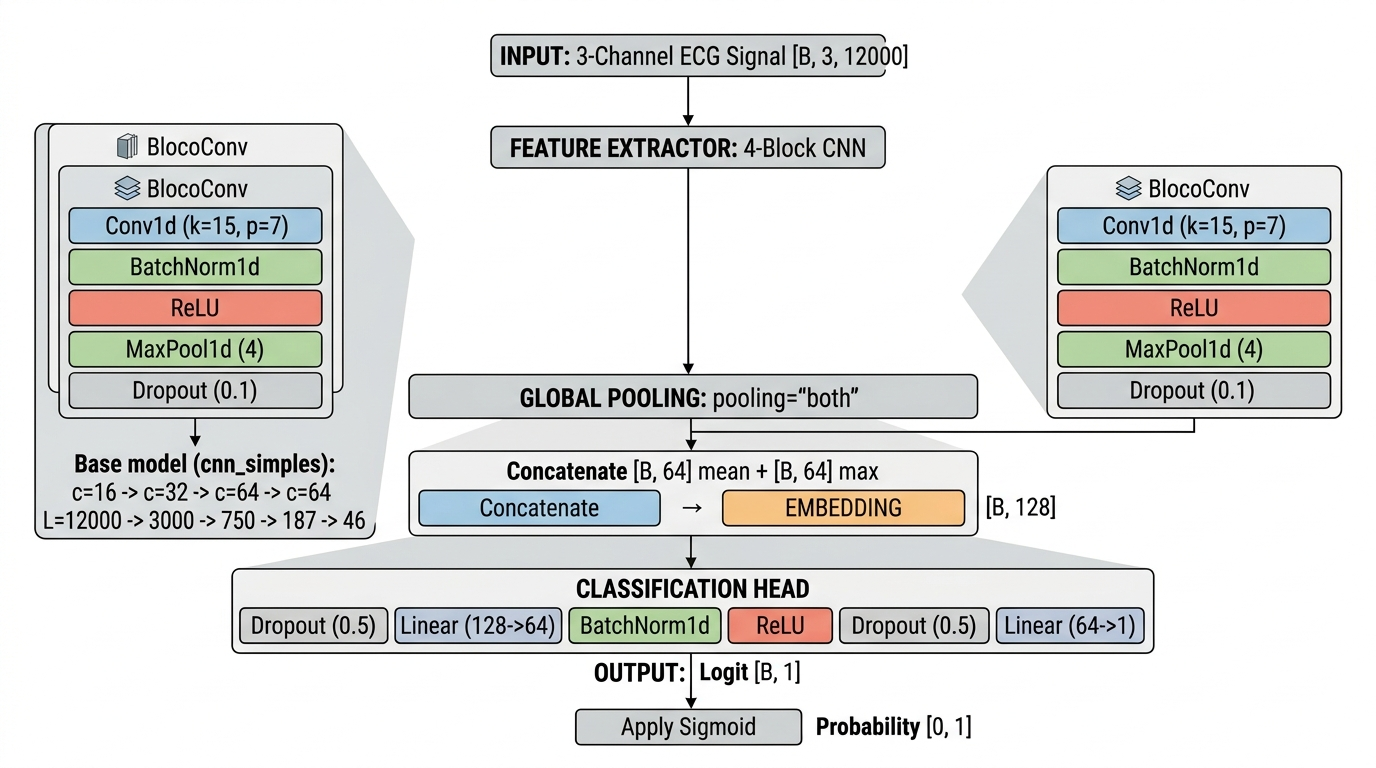
\includegraphics[width=16cm]{figuras/arquitetura_cnn.jpg}}
	}{
		\Fonte{elaborado pelo autor (2026).}
	}
\end{figure}

\subsubsection{Variantes de capacidade}
\label{subsubsec:fund-cnn-variantes}

Para avaliar se o desempenho depende da capacidade do modelo, a mesma
estrutura foi instanciada em três tamanhos, que diferem apenas no número de
blocos e de filtros por bloco. A variante \textit{mínima} tem três blocos,
com 8, 16 e 32 filtros; a \textit{simples}, quatro blocos, com 16, 32, 64 e
64 filtros; a \textit{média}, quatro blocos, com 32, 64, 128 e 128 filtros.
Todos os demais elementos --- largura do núcleo, agrupamento, descarte,
classificador e inicialização --- são idênticos. Entre a menor e a maior
variante, o número de parâmetros cresce cerca de 29 vezes. Se o desempenho
não acompanhar esse crescimento, a limitação não está na capacidade da
rede, mas na informação disponível nos dados.

A \autoref{tab:cnn-dimensoes} detalha os canais de cada variante e o
comprimento das representações intermediárias para as duas durações de
janela avaliadas: 2~minutos (24\,000 amostras) e 10~segundos (2\,000
amostras).

% ---- TABELA: dimensões ----
\begin{table}[h!]
	\captionsetup{width=15.5cm}
	\Caption{\label{tab:cnn-dimensoes} Canais e comprimento das
		representações intermediárias das variantes da rede convolucional}
	\IBGEtab{}{
		\begin{tabular}{lrrrrrr}
			\toprule
			                          & \multicolumn{3}{c}{Canais}          & \multicolumn{2}{c}{Comprimento} &                                         \\
			\cmidrule(lr){2-4} \cmidrule(lr){5-6}
			Etapa                     & \multicolumn{1}{c}{Mínima}          & \multicolumn{1}{c}{Simples}     &
			\multicolumn{1}{c}{Média} & \multicolumn{1}{c}{2 min}           &
			\multicolumn{1}{c}{10 s}  & \multicolumn{1}{c}{Campo receptivo}                                                                             \\
			\midrule \midrule
			Entrada                   & 3                                   & 3                               & 3   & 24\,000 & 2\,000 & 5\,ms          \\
			Bloco 1                   & 8                                   & 16                              & 32  & 6\,000  & 500    & 90\,ms         \\
			Bloco 2                   & 16                                  & 32                              & 64  & 1\,500  & 125    & 430\,ms        \\
			Bloco 3                   & 32                                  & 64                              & 128 & 375     & 31     & 1,8\,s         \\
			Bloco 4                   & ---                                 & 64                              & 128 & 93      & 7      & 7,2\,s         \\
			Agrupamento global        & 64                                  & 128                             & 256 & ---     & ---    & janela inteira \\
			\bottomrule
		\end{tabular}
	}{
		\Fonte{elaborado pelo autor (2026).}
	}
\end{table}

A coluna de campo receptivo indica a extensão do sinal original que
influencia cada posição de saída e não depende da duração da janela. Ao
final do primeiro bloco, cada posição reflete 90\,ms de registro ---
aproximadamente a duração de um complexo QRS ---; ao final do quarto,
7,2\,s, o equivalente a oito a nove ciclos cardíacos a 70\,bpm. A rede,
portanto, combina progressivamente padrões morfológicos de batimentos
isolados em padrões que abrangem sequências de batimentos.

A duração da janela altera o que esses padrões representam no conjunto.
Na janela de 2~minutos, o quarto bloco ainda produz 93 posições, cada uma
resumindo alguns segundos, e o agrupamento global combina dezenas de trechos
distintos. Na janela de 10~segundos, restam 7 posições cujo campo receptivo
já cobre a maior parte da janela, de modo que a rede analisa essencialmente
um único trecho de poucos batimentos. Na variante mínima, que não possui o
quarto bloco, o campo receptivo final é de 1,8\,s, cerca de dois ciclos
cardíacos.

\subsubsection{Largura do núcleo}
\label{subsubsec:fund-cnn-nucleo}

O núcleo convolucional foi dimensionado em $\kappa = 15$ amostras,
equivalentes a 75\,ms na frequência de 200\,Hz. A escolha difere da convenção
predominante em arquiteturas originadas no processamento de imagens, em que
núcleos de três elementos são usuais e corresponderiam, neste contexto, a
apenas 15\,ms. Com núcleo de 75\,ms, um único filtro da primeira camada
abrange parcela substancial de um complexo QRS, cuja duração normal situa-se
entre 80 e 100\,ms, podendo representar diretamente padrões de despolarização
ventricular.

\subsubsection{Agrupamento combinado}
\label{subsubsec:fund-cnn-pooling}

Ao término do último bloco, os canais são reduzidos a um vetor com o dobro
da sua dimensão pela concatenação dos agrupamentos globais por média e
máximo, conforme a \autoref{eq:pooling-global}: 64, 128 e 256 dimensões nas
variantes mínima, simples e média. As duas operações capturam aspectos
complementares: a média reflete o comportamento típico da janela, enquanto o
máximo registra o instante de maior ativação de cada filtro. A combinação
permite que a rede seja sensível tanto a alterações persistentes quanto a
eventos breves, como extrassístoles isoladas, que a média isoladamente
diluiria.

\subsubsection{Ausência de conexões residuais}
\label{subsubsec:fund-cnn-residual}

A arquitetura não emprega as conexões residuais descritas na
\autoref{sec:fund-resnet}. Essas conexões foram concebidas para viabilizar o
treinamento de redes com dezenas de camadas, nas quais o gradiente tenderia a
se atenuar ao percorrer a sequência de transformações. Com três ou quatro
blocos convolucionais, o gradiente alcança as camadas iniciais sem atenuação
significativa, e os atalhos acrescentariam parâmetros sem benefício
correspondente.

\subsubsection{Classificador e número de parâmetros}
\label{subsubsec:fund-cnn-classificador}

O vetor resultante do agrupamento alimenta um classificador composto por
duas camadas totalmente conectadas --- a primeira com 64 unidades,
normalização em lote e ativação \textit{ReLU}, a segunda com uma unidade de
saída ---, ambas precedidas por descarte com probabilidade 0,6. Os pesos das
camadas convolucionais são inicializados conforme \citeonline{he2015delving},
esquema adequado a redes com ativação \textit{ReLU}.

A \autoref{tab:cnn-parametros} decompõe os parâmetros treináveis de cada
variante. Como as camadas convolucionais não dependem do comprimento do
sinal, os valores são os mesmos para as duas durações de janela.

% ---- TABELA: parâmetros ----
\begin{table}[h!]
	\captionsetup{width=13.5cm}
	\Caption{\label{tab:cnn-parametros} Distribuição dos parâmetros das
		variantes da rede convolucional}
	\IBGEtab{}{
		\begin{tabular}{lrrr}
			\toprule
			Componente                  & \multicolumn{1}{c}{Mínima} &
			\multicolumn{1}{c}{Simples} & \multicolumn{1}{c}{Média}                        \\
			\midrule \midrule
			Bloco 1                     & 360                        & 720      & 1\,440   \\
			Bloco 2                     & 1\,920                     & 7\,680   & 30\,720  \\
			Bloco 3                     & 7\,680                     & 30\,720  & 122\,880 \\
			Bloco 4                     & ---                        & 61\,440  & 245\,760 \\
			Normalização dos blocos     & 112                        & 352      & 704      \\
			Classificador               & 4\,353                     & 8\,449   & 16\,641  \\
			\midrule
			Total                       & 14\,425                    & 109\,361 & 418\,145 \\
			Por paciente de treino      & 47                         & 354      & 1\,353   \\
			\bottomrule
		\end{tabular}
	}{
		\Fonte{elaborado pelo autor (2026).}
	}
\end{table}

Cada bloco convolucional tem $C \cdot C' \cdot \kappa$ pesos, sem termo de
viés, pois a normalização em lote seguinte o tornaria redundante. A última
linha divide o total pelos 309 pacientes do conjunto de treinamento de cada
partição. Mesmo a variante média tem cerca de dez vezes menos parâmetros por
paciente que a ResNet-18 descrita na \autoref{sec:fund-resnet}, que tem 3\,976\,385
parâmetros, ou 12\,869 por paciente de treinamento.

% arquitetura resnet =======================================


\subsection{Arquitetura das redes residuais}
\label{subsec:fund-resnet-arquitetura}

A arquitetura empregada adapta ao domínio unidimensional a estrutura proposta
por \citeonline{he2016deep}, seguindo a prática estabelecida em trabalhos de
classificação de \gls{ECG} com redes residuais
\cite{hannun2019cardiologist,ribeiro2020automatic}. Uma etapa inicial
precede quatro estágios de blocos residuais:

\begin{itemize}
	\item \textbf{Etapa inicial:} convolução com núcleo 7 e passo 2, seguida
	      de normalização em lote, \textit{ReLU} e agrupamento máximo com núcleo 3 e
	      passo 2. O comprimento é reduzido por quatro antes do primeiro bloco.
	\item \textbf{Estágios 1 a 4:} sequências de blocos residuais com $P$,
	      $2P$, $4P$ e $8P$ canais internos, em que $P$ denota a largura inicial.
	      O primeiro bloco dos estágios 2 a 4 emprega passo 2, dividindo o
	      comprimento pela metade e exigindo projeção no atalho.
	\item \textbf{Agrupamento global e classificador:} idênticos aos da
	      \autoref{subsec:fund-cnn-arquitetura}, com o vetor resultante de
	      dimensão $2 \times 8 \cdot P \cdot E$ ao combinar média e máximo.
\end{itemize}

A cada estágio, portanto, o comprimento temporal é dividido por dois e a
profundidade da representação, multiplicada por dois --- progressão distinta
da adotada na rede convolucional da \autoref{sec:fund-cnn}, que divide o
comprimento por quatro a cada bloco.

\subsubsection{Configurações avaliadas}
\label{subsubsec:fund-resnet-config}

Três parâmetros definem cada configuração: o tipo de bloco, o número de
blocos por estágio e a largura inicial $P$. A
\autoref{tab:resnet-configuracoes} reúne as quatro variantes avaliadas, que
percorrem uma faixa de dezesseis vezes em número de parâmetros.

% ---- TABELA: configurações ----
\begin{table}[h!]
	\captionsetup{width=15.5cm}
	\Caption{\label{tab:resnet-configuracoes} Configurações das redes
		residuais avaliadas}
	\IBGEtab{}{
		\begin{tabular}{lcccrr}
			\toprule
			Configuração              & Bloco                          & Blocos por estágio & $P$ &
			\multicolumn{1}{c}{Saída} & \multicolumn{1}{c}{Parâmetros}                                                    \\
			\midrule \midrule
			ResNet-18 reduzida        & básico                         & 2--2--2--2         & 32  & 256    & 1\,029\,985  \\
			ResNet-18 completa        & básico                         & 2--2--2--2         & 64  & 512    & 3\,976\,385  \\
			ResNet-34                 & básico                         & 3--4--6--3         & 64  & 512    & 7\,350\,721  \\
			ResNet-50                 & gargalo                        & 3--4--6--3         & 64  & 2\,048 & 16\,479\,937 \\
			\bottomrule
		\end{tabular}
	}{
		\Fonte{elaborado pelo autor (2026).}
	}
\end{table}

As configurações permitem examinar separadamente duas dimensões da
capacidade. A comparação entre as duas variantes da ResNet-18 isola o efeito
da \textit{largura}: mesma profundidade, o dobro de canais. A comparação
entre a ResNet-18 completa e a ResNet-34 isola o efeito da
\textit{profundidade}: mesma largura, o dobro de blocos. A ResNet-50 combina
a profundidade da ResNet-34 com o bloco de gargalo e saída quatro vezes mais
larga.

Os números de parâmetros são inferiores aos das versões bidimensionais
homônimas, nas quais a ResNet-18 possui cerca de 11 milhões, porque o núcleo
unidimensional de largura três contém três pesos por par de canais, contra
nove do núcleo $3 \times 3$.

\subsubsection{Dimensões e campo receptivo}
\label{subsubsec:fund-resnet-dimensoes}

A \autoref{tab:resnet-dimensoes} apresenta as dimensões das representações
intermediárias para a janela de 24\,000 amostras e o campo receptivo ao
término de cada etapa.

% ---- TABELA: dimensões ----
\begin{table}[h!]
	\captionsetup{width=15.5cm}
	\Caption{\label{tab:resnet-dimensoes} Dimensões e campo receptivo das
		redes residuais para janela de 24\,000 amostras}
	\IBGEtab{}{
		\begin{tabular}{lrrrrr}
			\toprule
			                              &                                 & \multicolumn{2}{c}{Canais} & \multicolumn{2}{c}{Campo receptivo}                     \\
			\cmidrule(lr){3-4} \cmidrule(lr){5-6}
			Etapa                         & \multicolumn{1}{c}{Comprimento} &
			\multicolumn{1}{c}{18 e 34}   & \multicolumn{1}{c}{50}          &
			\multicolumn{1}{c}{ResNet-18} & \multicolumn{1}{c}{ResNet-34}                                                                                          \\
			\midrule \midrule
			Entrada                       & 24\,000                         & 3                          & 3                                   & 5\,ms   & 5\,ms   \\
			Etapa inicial                 & 6\,000                          & 64                         & 64                                  & 55\,ms  & 55\,ms  \\
			Estágio 1                     & 6\,000                          & 64                         & 256                                 & 215\,ms & 295\,ms \\
			Estágio 2                     & 3\,000                          & 128                        & 512                                 & 495\,ms & 895\,ms \\
			Estágio 3                     & 1\,500                          & 256                        & 1\,024                              & 1,1\,s  & 2,7\,s  \\
			Estágio 4                     & 750                             & 512                        & 2\,048                              & 2,2\,s  & 4,5\,s  \\
			\bottomrule
		\end{tabular}
	}{
		\Fonte{elaborado pelo autor (2026).}
	}
\end{table}

O campo receptivo ao final da ResNet-18 é de 2,2\,s --- inferior aos 7,2\,s da
rede convolucional rasa, apesar de esta possuir apenas quatro camadas
convolucionais contra dezessete. A diferença decorre do núcleo: com três
amostras (15\,ms), cada convolução residual amplia pouco a extensão
observada, e a cobertura temporal depende do empilhamento de muitas camadas.
A ResNet-34, com o dobro de blocos, alcança 4,5\,s. A ResNet-50 apresenta
campo receptivo semelhante ao da ResNet-18, pois apenas uma das três
convoluções de cada bloco de gargalo considera vizinhança temporal.

Ainda que inferior à duração da janela, esse campo receptivo não limita a
informação disponível ao classificador: o agrupamento global da
\autoref{eq:pooling-global} combina as 750 posições do último estágio,
abrangendo os dois minutos integralmente.

\subsubsection{Distribuição dos parâmetros}
\label{subsubsec:fund-resnet-parametros}

Os parâmetros concentram-se nos estágios finais, em que o número de canais é
maior. Na ResNet-18 completa, o quarto estágio, com 512 canais, responde por
aproximadamente três quartos do total. Na ResNet-50, o classificador recebe
vetor de 4\,096 dimensões --- 2\,048 de cada agrupamento ---, e sua primeira
camada sozinha possui cerca de 525\,000 parâmetros.

Os pesos das camadas convolucionais são inicializados conforme
\citeonline{he2015delving}, e os parâmetros de escala e deslocamento da
normalização em lote, com um e zero, respectivamente, de modo que cada bloco
inicie próximo da identidade.

\subsection{Regime de dados das redes residuais}
\label{subsec:fund-resnet-regime}

As redes residuais foram concebidas para conjuntos de treinamento de grande
porte. A ResNet original foi avaliada sobre 1,28 milhão de imagens
\cite{he2016deep}; no domínio do \gls{ECG}, os trabalhos que estabeleceram
seu desempenho empregaram dezenas de milhares a milhões de registros
\cite{hannun2019cardiologist,ribeiro2020automatic}.

Neste trabalho, cada partição dispõe de 309 pacientes no treinamento, dos
quais 33 casos. A razão entre parâmetros e pacientes varia de $3\,333$ na
ResNet-18 reduzida a cerca de $53\,000$ na ResNet-50. Nesse regime, a
capacidade da rede é amplamente suficiente para ajustar individualmente cada
exemplo de treinamento, o que motiva a comparação sistemática entre
configurações de capacidade crescente apresentada no
\autoref{cap:resultados}: se a capacidade fosse o fator limitante, o
desempenho deveria variar com ela.


\subsection{Arquitetura da rede residual com atenção}
\label{subsec:fund-atencao-arquitetura}

A arquitetura avaliada mantém integralmente o corpo da ResNet-18 reduzida
(\autoref{tab:resnet-configuracoes}), que produz sequência de 750 posições
com 256 canais, e insere entre ele e o agrupamento global uma camada
codificadora com os parâmetros da \autoref{tab:atencao-config}.

% ---- TABELA: configuração ----
\begin{table}[h!]
	\captionsetup{width=12cm}
	\Caption{\label{tab:atencao-config} Configuração da camada de atenção}
	\IBGEtab{}{
		\begin{tabular}{ll}
			\toprule
			Parâmetro & Valor \\
			\midrule \midrule
			Comprimento da sequência ($L$) & 750 posições \\
			Dimensão do modelo ($d$) & 256 \\
			Número de cabeças ($h$) & 4 \\
			Dimensão por cabeça ($d_k$) & 64 \\
			Dimensão da rede interna ($d_{\mathrm{ff}}$) & 512 \\
			Número de camadas & 1 \\
			Descarte & 0,3 \\
			\bottomrule
		\end{tabular}
	}{
	\Fonte{elaborado pelo autor (2026).}
}
\end{table}

A saída do codificador, com as mesmas dimensões da entrada, passa pelo
agrupamento global combinado de média e máximo, resultando em vetor de 512
dimensões. Diferentemente das demais redes, o classificador consiste em uma
única camada linear precedida de descarte, sem camada intermediária: a
capacidade adicional introduzida pela atenção dispensa a não linearidade
extra no classificador.

A \autoref{tab:atencao-parametros} decompõe os parâmetros.

% ---- TABELA: parâmetros ----
\begin{table}[h!]
	\captionsetup{width=12.5cm}
	\Caption{\label{tab:atencao-parametros} Distribuição dos parâmetros da
	ResNet-18 reduzida com camada de atenção}
	\IBGEtab{}{
		\begin{tabular}{lrr}
			\toprule
			Componente & \multicolumn{1}{c}{Parâmetros} &
			\multicolumn{1}{c}{Fração} \\
			\midrule \midrule
			Corpo residual & 963\,936 & 64,6\,\% \\
			Atenção com múltiplas cabeças & 263\,168 & 17,6\,\% \\
			Rede interna (FFN) & 262\,912 & 17,6\,\% \\
			Normalização de camada & 1\,024 & 0,1\,\% \\
			Classificador & 513 & $<$\,0,1\,\% \\
			\midrule
			Total & 1\,491\,553 & 100,0\,\% \\
			\bottomrule
		\end{tabular}
	}{
	\Fonte{elaborado pelo autor (2026).}
}
\end{table}

A camada de atenção acrescenta $527\,104$ parâmetros, cerca de metade do
corpo convolucional e 35\,\% do total.

\subsubsection{Ausência de codificação posicional}
\label{subsubsec:fund-posicional}

A operação da \autoref{eq:atencao} é invariante à ordem das posições: se a
sequência de entrada for permutada, a saída é permutada da mesma forma. Em
aplicações nas quais a ordem é essencial, como a linguagem, acrescenta-se à
entrada uma \textit{codificação posicional} que identifica cada posição
\cite{vaswani2017attention}.

A arquitetura empregada não utiliza codificação posicional. Duas razões
sustentam a escolha. A primeira é que as representações produzidas pelo
corpo convolucional já carregam informação local de ordem, pois cada posição
resume um trecho contíguo do sinal. A segunda é que a saída do codificador é
submetida ao agrupamento global, operação também invariante à ordem: a
posição absoluta de um padrão dentro da janela de dois minutos não altera a
representação final. O que a atenção acrescenta, nesse arranjo, é a
possibilidade de cada posição ser representada em função do conteúdo das
demais, e não a modelagem da ordem temporal propriamente dita.

\subsection{Regime de dados da rede com atenção}
\label{subsec:fund-atencao-regime}

As arquiteturas baseadas em atenção apresentam menos vieses indutivos que
as convolucionais. Uma convolução pressupõe, por construção, que padrões
relevantes são locais e podem ocorrer em qualquer posição; a atenção não
pressupõe localidade e precisa aprender, a partir dos dados, quais relações
são relevantes. \citeonline{dosovitskiy2021image} mostraram que essa
flexibilidade só se converte em vantagem quando o conjunto de treinamento é
suficientemente grande: em conjuntos de pequeno porte, modelos baseados em
atenção apresentaram desempenho inferior ao de redes convolucionais de
capacidade semelhante.

A arquitetura híbrida aqui empregada atenua esse problema ao preservar o
corpo convolucional e restringir a atenção a uma única camada sobre
representações já comprimidas. Ainda assim, com 33 casos positivos por
partição de treinamento, a estimativa dos $527\,104$ parâmetros adicionais
encontra-se no regime em que a literatura reporta menor eficácia do
mecanismo.


\section{Cenário I: treinamento e avaliação das redes}
\label{sec:configuracao-experimental}


As arquiteturas avaliadas nas seções seguintes compartilham o mesmo
protocolo de preparação dos dados, treinamento e avaliação. Essa
uniformidade é condição para que a comparação entre elas isole o efeito da
arquitetura, e não o de escolhas acessórias de configuração. Os valores
adotados foram fixados a partir das primeiras execuções e mantidos ao longo
dos experimentos; são apresentados a seguir, acompanhados da justificativa
correspondente. Duas configurações foram empregadas: a das redes residuais,
de atenção e com concatenação, e a das redes convolucionais, que estendeu o número
de épocas e de janelas. As diferenças entre elas são indicadas nas tabelas.


\subsection{Representação do sinal}
\label{subsec:config-sinal}

Cada paciente é representado por janelas extraídas de seu registro de
24\,horas, e não pelo registro integral. A opção decorre de uma limitação
prática: a 200\,Hz, três derivações durante 24\,horas correspondem a
aproximadamente 17 milhões de amostras por paciente, volume incompatível com
o processamento em lote na memória disponível.

A \autoref{tab:config-sinal} reúne os parâmetros de representação.

% ---- TABELA: parâmetros do sinal ----
\begin{table}[h!]
	\captionsetup{width=14cm}
	\Caption{\label{tab:config-sinal} Parâmetros de representação do sinal}
	\IBGEtab{}{
		\begin{tabular}{lll}
			\toprule
			Parâmetro                        & Valor                      & Justificativa                        \\
			\midrule \midrule
			Comprimento da janela            & 24\,000 amostras           & 2 min, cerca de 140 ciclos cardíacos \\
			Janelas por paciente (treino)    & 250 / 350 & posições sorteadas a cada época      \\
			Janelas por paciente (avaliação) & 100 / 200 & posições em grade fixa               \\
			Margem descartada                & 5 min                      & calibração do equipamento            \\
			Filtro passa-banda               & 0,5--40\,Hz                & remove deriva e ruído muscular       \\
			Normalização                     & percentil 99 por derivação & preserva amplitude relativa          \\
			Limitação de amplitude           & $[-5, 5]$                  & atenua artefatos de movimento        \\
			\bottomrule
		\end{tabular}
	}{
		\Fonte{elaborado pelo autor (2026). Nota: quando há dois valores, o primeiro
			refere-se às redes residuais, de atenção e com concatenação, e o segundo, às redes
			convolucionais.}
	}
\end{table}

A janela de dois minutos abrange aproximadamente 140 ciclos cardíacos a uma
frequência de 70\,bpm, quantidade suficiente para que a morfologia se repita
e para que a variabilidade entre batimentos seja observável. Janelas mais
curtas podem recair sobre trechos sem conteúdo relevante; janelas mais longas
elevam o consumo de memória e reduzem o número de amostras disponíveis por
paciente.

No treinamento, as posições das janelas são sorteadas a cada época,
funcionando como forma de aumento de dados: o modelo nunca observa
exatamente o mesmo recorte duas vezes. Na avaliação, as posições seguem grade
regular determinística, assegurando reprodutibilidade das métricas.

A separação entre filtragem e normalização é deliberada. O filtro
passa-banda remove o deslocamento de linha de base de cada janela
individualmente --- deslocamento que varia entre pacientes conforme o
posicionamento dos eletrodos. A escala,
por sua vez, é estimada uma única vez sobre o conjunto de treinamento de cada
partição, de modo idêntico para todos os pacientes, o que preserva as
diferenças de amplitude entre indivíduos --- informação associada a condições
como baixa voltagem e hipertrofia ventricular. A padronização por janela,
alternativa descartada, executaria as duas operações simultaneamente e
eliminaria essa informação.

\subsection{Treinamento}
\label{subsec:config-treino}

A \autoref{tab:config-treino} apresenta os hiperparâmetros de otimização,
comuns a todas as arquiteturas, salvo o número de épocas e a paciência.

% ---- TABELA: hiperparâmetros de treino ----
\begin{table}[h!]
	\captionsetup{width=14cm}
	\Caption{\label{tab:config-treino} Hiperparâmetros de treinamento}
	\IBGEtab{}{
		\begin{tabular}{lll}
			\toprule
			Parâmetro                 & Valor                  & Justificativa                          \\
			\midrule \midrule
			Otimizador                & AdamW                  & desacopla regularização do gradiente   \\
			Taxa de aprendizado       & $1{,}0 \times 10^{-4}$ & valores maiores causaram instabilidade \\
			Regularização ($\lambda$) & $1{,}0 \times 10^{-2}$ & limite superior usual                  \\
			Descarte                  & 0,6                    & compensa a razão parâmetros/eventos    \\
			Tamanho do lote           & 256\footnotemark[1]    &                                        \\
			Épocas máximas            & 20 / 30 & melhor época ocorreu cedo            \\
			Paciência                 & 10 / 15 & sobre média móvel de três            \\
			Agrupamento               & média e máximo         & estado típico e instante extremo       \\
			Precisão                  & mista (fp16)           & reduz consumo de memória               \\
			\bottomrule
		\end{tabular}
	}{
		\Fonte{elaborado pelo autor (2026). Nota: em épocas e paciência, o primeiro valor
			refere-se às redes residuais, de atenção e com concatenação, e o segundo, às redes
			convolucionais.}
	}
\end{table}

\footnotetext[1]{Reduzido para 128 na ResNet-50 por limitação de memória da
	unidade de processamento gráfico.}

Os valores de regularização e descarte situam-se no extremo superior das
faixas habituais. A escolha decorre da razão entre o número de parâmetros e
o de eventos disponíveis: mesmo a arquitetura mais enxuta avaliada dispõe de
$14\,425$ parâmetros para 33 casos positivos no conjunto de treinamento de
cada partição, e as redes residuais, de milhões. Nas primeiras execuções,
valores menores de regularização produziram perdas de treinamento próximas
de zero já na terceira época.

O limite de 20 ou 30 épocas acompanha a observação, recorrente em todas as
arquiteturas, de que o melhor valor de \gls{AUC} sobre o conjunto de
validação ocorre nas primeiras épocas. O critério de parada emprega média
móvel de três épocas em lugar do valor pontual: com apenas 11 eventos no
conjunto de validação, a métrica de uma única época oscila substancialmente
sem que o modelo tenha se alterado de forma apreciável, e a suavização evita
que se selecione o pico do ruído.

\subsection{Desbalanceamento entre classes}
\label{subsec:config-desbalanceamento}

Com prevalência de 10,6\,\%, um classificador que atribua a classe
majoritária a todos os pacientes alcança acurácia de 89,4\,\% com
sensibilidade nula. Para evitar a convergência a esse ótimo local, a função
de perda de entropia cruzada binária foi ponderada pelo fator

\begin{equation}
	w_{+} = \frac{N_0}{N_1} \approx 8{,}4,
	\label{eq:pos-weight}
\end{equation}

\noindent
em que $N_0$ e $N_1$ denotam, respectivamente, o número de controles e de
casos no conjunto de treinamento de cada partição. O fator multiplica a
contribuição dos casos positivos ao gradiente, sendo equivalente a replicar
cada evento cerca de 8,4 vezes sem descartar controles.

Técnicas de subamostragem da classe majoritária foram descartadas: o
equilíbrio entre classes seria obtido às custas de reduzir a coorte de 517
para 110 pacientes, sem alterar o número de eventos --- que constitui o
fator efetivamente limitante --- e com ampliação dos intervalos de confiança.


\subsection{Experimentos com a rede convolucional}
\label{subsec:met-cnn-experimentos}

A rede convolucional descrita na \autoref{subsec:fund-cnn-arquitetura} foi
avaliada em um delineamento fatorial com dois fatores: a capacidade do
modelo, nas variantes mínima, simples e média, e a duração da janela de
entrada, de 2~minutos e de 10~segundos. As seis combinações resultantes,
listadas na \autoref{tab:met-cnn-experimentos}, foram treinadas sob
configuração idêntica, de modo que as diferenças de desempenho possam ser
atribuídas apenas a esses dois fatores.

\begin{table}[h!]
	\captionsetup{width=12cm}
	\Caption{\label{tab:met-cnn-experimentos} Combinações avaliadas da rede
		convolucional}
	\IBGEtab{}{
		\begin{tabular}{lrrr}
			\toprule
			Variante                            & \multicolumn{1}{c}{Parâmetros} &
			\multicolumn{1}{c}{Janela de 2 min} &
			\multicolumn{1}{c}{Janela de 10 s}                                             \\
			\midrule \midrule
			Mínima                              & 14\,425                        & E1 & E4 \\
			Simples                             & 109\,361                       & E2 & E5 \\
			Média                               & 418\,145                       & E3 & E6 \\
			\bottomrule
		\end{tabular}
	}{
		\Fonte{elaborado pelo autor (2026).}
	}
\end{table}

\subsubsection{Amostragem das janelas}

No treinamento, cada paciente contribui com o mesmo número de janelas por
época nas duas durações. Desse modo, as seis configurações recebem o mesmo
número de atualizações de gradiente, e o que varia entre as janelas de
2~minutos e de 10~segundos é apenas o conteúdo de cada exemplo. As janelas
de um paciente são sorteadas a cada época entre blocos consecutivos e sem
sobreposição do registro, descartados os 5~minutos iniciais e finais. A
permutação dos blocos é determinada pelo paciente e pela época, o que
garante que duas janelas do mesmo paciente nunca se sobreponham dentro de
uma época e que épocas sucessivas percorram trechos diferentes do exame.

Na avaliação, as janelas são posicionadas em uma grade fixa e uniforme ao
longo do registro, o que torna a predição reprodutível. São avaliadas 200 janelas
por paciente nas duas durações, o que corresponde a cerca de 6,7~horas de
registro com a janela de 2~minutos e a cerca de 33~minutos com a de
10~segundos.

\subsubsection{Filtragem com margem}

O filtro passa-faixa descrito na \autoref{sec:met-preprocessamento} requer
alguns segundos de sinal para estabilizar e, quando aplicado a um trecho
curto, distorce suas extremidades. Para evitar esse efeito, cada janela é
lida com 5~segundos adicionais de cada lado, filtrada e, em seguida,
recortada no comprimento nominal. A rede recebe, assim, exatamente 24\,000 ou
2\,000 amostras livres do transitório de borda, o que é particularmente
relevante para a janela de 10~segundos, na qual as margens distorcidas
representariam fração apreciável do sinal.

\subsubsection{Configuração comum}

As seis configurações compartilham a validação cruzada em cinco partições
estratificadas por paciente, com 25\,\% do conjunto de treinamento de cada
partição reservado para validação interna (309 ou 310 pacientes de
treinamento por partição), a função de perda ponderada da
\autoref{eq:bce-ponderada}, o otimizador AdamW com taxa de aprendizado de
$10^{-4}$ e decaimento de pesos de $10^{-2}$, lotes de 256 janelas e
no máximo 30 épocas, com interrupção antecipada após 15 épocas sem melhora. Em cada época, cada paciente contribui com 350 janelas de treinamento.
A probabilidade de cada paciente é a média das probabilidades de suas
janelas, e o limiar de decisão é escolhido pelo índice de Youden na
validação interna, nunca no conjunto de teste.



\subsection{Protocolo de treinamento e avaliação}
\label{subsec:met-protocolo-redes}

Todas as redes foram treinadas e avaliadas pelo mesmo procedimento,
resumido na \autoref{fig:met-protocolo} e detalhado a seguir. Os
hiperparâmetros constam da \autoref{tab:config-treino}.

% ---- FIGURA: fluxo do protocolo em uma partição ----
% Sugestão de conteúdo (uma caixa por etapa, da esquerda para a direita):
%   517 pacientes -> 5 partições estratificadas -> [partição k]
%   treino (75%) | validação interna (25%) | teste
%   -> estatísticas só no treino -> épocas: treino / validação / AUC suavizada
%   -> melhor época -> limiar de Youden na validação -> teste
%   -> predições fora da partição dos 517 -> AUC agrupada + IC bootstrap
% \begin{figure}[h!]
% 	\captionsetup{width=16cm}
% 	\Caption{\label{fig:met-protocolo} Protocolo de treinamento e avaliação
% 		em uma partição da validação cruzada}
% 	\UFCfig{}{
% 		\fbox{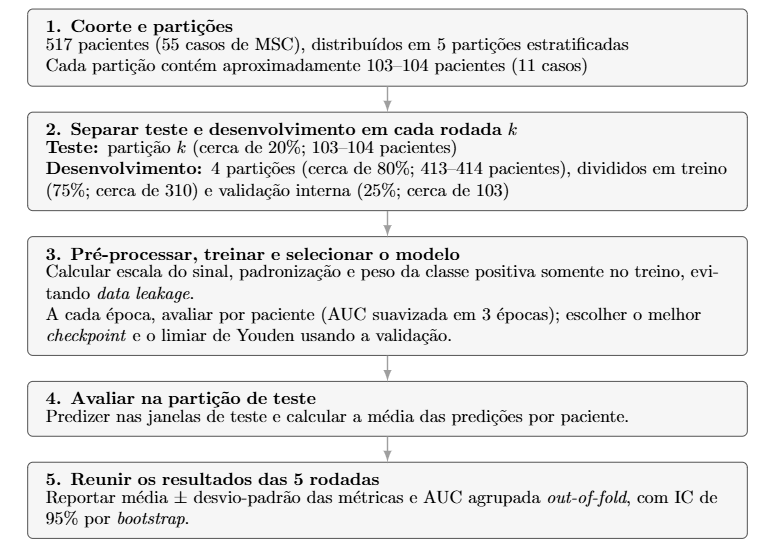
\includegraphics[width=16cm]{figuras/protocolo_validacao.png}}
% 	}{
% 		\Fonte{elaborado pelo autor (2026).}
% 	}
% \end{figure}

\begin{figure}[htbp]
	\centering
	\begin{tikzpicture}[
		step/.style={rectangle, rounded corners=3pt, draw=#1!65!black,
				fill=#1!7, text width=0.82\linewidth, align=left,
				inner xsep=10pt, inner ysep=6pt, font=\small},
		flow/.style={-{Latex[length=2.2mm]}, draw=gray!75, line width=0.8pt},
		node distance=5mm
		]
		\node[step=gray] (cohort) {\textbf{1. Coorte e partições}\\[-2pt]
			517 pacientes (55 casos de MSC), distribuídos em 5 partições estratificadas\\
			Cada partição contém aproximadamente 103--104 pacientes (11 casos)};

		\node[step=gray, below=of cohort] (split) {\textbf{2. Separar teste e desenvolvimento em cada rodada $k$}\\[-2pt]
			\textbf{Teste:} partição $k$ (cerca de 20\%; 103--104 pacientes)\\
			\textbf{Desenvolvimento:} 4 partições (cerca de 80\%; 413--414 pacientes), divididos em treino (75\%; cerca de 310) e validação interna (25\%; cerca de 103)};

		\node[step=gray, below=of split] (model) {\textbf{3. Pré-processar, treinar e selecionar o modelo}\\[-2pt]
			Calcular escala do sinal, padronização e peso da classe positiva somente no treino, evitando \textit{data leakage}.\\
			A cada época, avaliar por paciente (AUC suavizada em 3 épocas); escolher o melhor \textit{checkpoint} e o limiar de Youden usando a validação.};

		\node[step=gray, below=of model] (test) {\textbf{4. Avaliar na partição de teste}\\[-2pt]
			Predizer nas janelas de teste e calcular a média das predições por paciente.};

		\node[step=gray, below=of test] (results) {\textbf{5. Reunir os resultados das 5 rodadas}\\[-2pt]
			Reportar média $\pm$ desvio-padrão das métricas e AUC agrupada \textit{out-of-fold}, com IC de 95\% por \textit{bootstrap}.};

		\draw[flow] (cohort) -- (split);
		\draw[flow] (split) -- (model);
		\draw[flow] (model) -- (test);
		\draw[flow] (test) -- (results);
	\end{tikzpicture}
	\caption{Fluxo da validação cruzada estratificada em 5 partições. As etapas 2--4 são repetidas para cada partição, com avaliação no nível do paciente.}
	\label{fig:met-protocolo}
\end{figure}



\subsubsection{Divisão dos pacientes}

Os 517 pacientes foram divididos em cinco partições estratificadas, com 103
ou 104 pacientes e 11 casos cada uma. Em cada rodada, uma partição forma o
conjunto de teste e as outras quatro, o conjunto de desenvolvimento. Deste,
25\,\% dos pacientes, também por sorteio estratificado, formam a validação
interna, e os 75\,\% restantes, o treinamento --- 309 ou 310 pacientes, dos
quais 33 casos. A validação interna é usada para escolher a época do modelo
e o limiar de decisão; o conjunto de teste não participa de nenhuma escolha.

A cada rodada, as estatísticas que dependem dos dados --- a escala do sinal
por derivação, as médias e desvios das variáveis clínicas e o peso da classe
positiva, $w_{+} = N_0/N_1 \approx 8{,}4$ --- são recalculadas com os
pacientes de treinamento daquela rodada.

\subsubsection{Seleção da época}

Ao final de cada época, a rede prediz as janelas da validação interna, as
probabilidades são agregadas por paciente, e calcula-se a \gls{AUC}. Como a
validação contém apenas 11 casos, a \gls{AUC} de uma única época oscila
consideravelmente sem que o modelo tenha mudado de forma relevante. Por isso,
o critério de seleção é a média móvel da \gls{AUC} nas três últimas épocas:
os pesos são salvos sempre que essa média supera o melhor valor anterior, e
o treinamento é interrompido quando ela deixa de melhorar por um número
pré-definido de épocas.

A taxa de aprendizado decai ao longo das épocas segundo uma função cosseno
\cite{loshchilov2017sgdr}. Ela parte do valor inicial $\eta_{\max} =
10^{-4}$ e diminui suavemente até próximo de zero na última época prevista:

\begin{equation}
	\eta_t = \frac{\eta_{\max}}{2}\left(1 + \cos\frac{\pi\, t}{T}\right),
	\label{eq:cosseno}
\end{equation}

\noindent
em que $\eta_t$ é a taxa de aprendizado na época $t$ e $T$ é o número máximo
de épocas. O decaimento permite passos maiores no início do treinamento,
quando a rede ainda está longe de uma boa solução, e ajustes finos no fim.
Com a parada antecipada, o treinamento costuma ser interrompido antes de a
taxa chegar a zero.

\subsubsection{Avaliação no teste}

Concluído o treinamento, os pesos da melhor época são restaurados. O limiar
de decisão é obtido pelo índice de Youden (\autoref{eq:youden}) sobre as
predições da validação interna e aplicado, sem alteração, ao conjunto de
teste. Para cada paciente de teste, a probabilidade é a média das
probabilidades de suas janelas.

\subsubsection{Consolidação das cinco rodadas}

Os resultados de cada arquitetura são reportados de duas formas
complementares. A primeira é a média e o desvio-padrão das métricas das
cinco partições, que indicam a estabilidade do modelo: desvios elevados
sinalizam que o resultado depende de quais pacientes caíram em cada
partição. A segunda reúne as predições fora da partição dos 517 pacientes em
uma única curva ROC, cuja \gls{AUC} recebe um intervalo de confiança de
95\,\% por \textit{bootstrap} com $B^{*} = 1\,000$ reamostragens de
pacientes. Para as métricas dependentes de limiar dessa curva agrupada,
emprega-se a mediana dos cinco limiares obtidos nas validações internas.

Como análise secundária, registra-se também a \gls{AUC} obtida quando a
probabilidade do paciente é a máxima, e não a média, de suas janelas, o que
privilegia a janela de maior risco ao longo do registro.



\section{Cenário II: extração de características do ECG}
\label{sec:met-cenario2}
\label{sec:met-extracao}

No segundo cenário, o sinal do Holter passa por pré-processamento e extração
de características, e as medidas obtidas --- os marcadores
eletrocardiográficos --- são a entrada de modelos de aprendizado de máquina
clássico. Os marcadores descritos na \autoref{sec:fund-marcadores} foram extraídos dos
registros de Holter dos 517 pacientes da coorte segundo dois protocolos,
que diferem na duração e na densidade dos segmentos analisados. O protocolo
A privilegia segmentos longos, que permitem a análise espectral; o protocolo
B adota segmentos curtos e densos, que permitem acompanhar o ritmo ao longo
do dia, seguindo o desenho de \citeonline{swee2026multimodal}. A
\autoref{tab:met-protocolos} resume as diferenças. Ambos empregam o mesmo
filtro passa-faixa das redes neurais (\autoref{sec:met-preprocessamento}) e
a biblioteca NeuroKit2 \cite{makowski2021neurokit2} para a detecção de picos
e a delineação dos batimentos.

\begin{table}[h!]
	\captionsetup{width=15cm}
	\Caption{\label{tab:met-protocolos} Protocolos de extração dos marcadores}
	\IBGEtab{}{
		\begin{tabular}{lll}
			\toprule
			                       & Protocolo A                 & Protocolo B                  \\
			\midrule \midrule
			Segmento               & 5 minutos                   & 30 segundos                  \\
			Espaçamento            & um segmento por hora        & um segmento a cada 2 minutos \\
			Margem descartada      & 1 hora em cada extremidade  & 1 hora em cada extremidade   \\
			Segmentos por paciente & cerca de 21                 & cerca de 636 (máximo de 660) \\
			Tempo analisado        & cerca de 1 h 45 min         & cerca de 5 h 20 min          \\
			Derivação              & a de maior amplitude        & Y                            \\
			Correção de artefatos  & sim                         & não                          \\
			Base da \gls{VFC}      & intervalos RR filtrados     & intervalos NN                \\
			Domínio da frequência  & sim                         & não                          \\
			Indicadores de ectopia & proporção de RR irregulares & contagens completas          \\
			\bottomrule
		\end{tabular}
	}{
		\Fonte{elaborado pelo autor (2026). Segmentos e tempo analisado por
			paciente, sobre as cerca de 22~horas úteis de cada registro: no
			protocolo A, um segmento de 5~minutos no início de cada hora; no
			protocolo B, um segmento de 30~segundos a cada 2~minutos (total de
			328\,807 segmentos nos 517 pacientes).}
	}
\end{table}

\subsection{Marcadores extraídos}
\label{subsec:met-marcadores-extraidos}

A \autoref{tab:fund-biomarcadores} reúne os marcadores extraídos neste
trabalho, com sua definição, unidade e significado fisiológico. Cada um é
calculado em cada segmento e depois resumido por paciente de duas formas: a
média entre os segmentos, que representa o nível típico do marcador, e o
desvio-padrão entre os segmentos, que representa quanto ele varia ao longo
do dia. Assim, o desvio-padrão da frequência cardíaca média, por exemplo, não
mede a variação batimento a batimento, mas a diferença de frequência entre os
períodos do registro, incluindo o ciclo dia--noite.

\begin{table}[h!]
	\captionsetup{width=16cm}
	\Caption{\label{tab:fund-biomarcadores} Marcadores eletrocardiográficos
		extraídos: definição e significado}
	\IBGEtab{}{
		\footnotesize
		\begin{tabular}{p{3.3cm}p{5.6cm}p{1.1cm}p{5.2cm}}
			\toprule
			Marcador & Definição & Unidade & Significado \\
			\midrule \midrule
			\multicolumn{4}{l}{\textit{Ritmo e variabilidade (sobre intervalos NN)}} \\
			Frequência cardíaca média & 60\,000 dividido pela média dos intervalos NN & bpm & Nível de ativação do ritmo \\
			Intervalo RR médio & Média dos intervalos NN & ms & Inverso da frequência \\
			\gls{SDNN} & Desvio-padrão dos intervalos NN (\autoref{eq:sdnn}) & ms & Variabilidade total do segmento \\
			\gls{RMSSD} & Raiz da média dos quadrados das diferenças sucessivas (\autoref{eq:rmssd}) & ms & Variação batimento a batimento; tônus vagal \\
			\gls{pNN50} & Porcentagem de diferenças sucessivas maiores que 50\,ms & \% & Tônus vagal \\
			SD1 e SD2 & Dispersões do gráfico de Poincaré (\autoref{eq:poincare}) & ms & Variabilidade de curto e de longo prazo \\
			SD1/SD2 & Razão entre as duas dispersões & --- & Forma da nuvem de Poincaré \\
			\gls{VLF}, \gls{LF}, \gls{HF}, LF/HF & Potência espectral por faixa (só em 5~minutos) & u.a.$^{a}$ & Modulação autonômica por mecanismo \\
			Entropia amostral & Regularidade da sequência de intervalos (só em 5~minutos) & --- & Complexidade do ritmo \\
			\midrule
			\multicolumn{4}{l}{\textit{Ectopia e pausas (pelo ritmo, sem distinguir a origem)}} \\
			Batimentos precoces & Intervalos RR menores que 80\,\% da mediana local & contagem & Batimentos fora do ritmo sinusal \\
			Extrassístoles & Precoce seguido de intervalo maior que 115\,\% da mediana local & contagem & Batimento ectópico com pausa compensatória \\
			Dupletes & Dois intervalos precoces consecutivos & contagem & Ectopia repetitiva; instabilidade elétrica \\
			Carga de ectopia & Porcentagem de intervalos precoces & \% & Frequência global de ectopia \\
			Intervalos irregulares & Porcentagem de intervalos plausíveis que não são NN & \% & Irregularidade do ritmo \\
			Maior pausa & Maior intervalo RR plausível do segmento & ms & Pausas e bradiarritmias \\
			Pausas acima de 2\,s & Intervalos RR maiores que 2\,000\,ms & contagem & Pausas prolongadas \\
			\midrule
			\multicolumn{4}{l}{\textit{Morfologia (mediana dos batimentos delineados)}} \\
			Duração do QRS & Do início ao fim do complexo QRS & ms & Condução ventricular; bloqueios de ramo \\
			Intervalo \gls{QT} & Do início do QRS ao fim da onda T & ms & Despolarização e repolarização ventriculares \\
			\gls{QTc} & QT corrigido pela frequência (\autoref{eq:bazett}) & ms & Repolarização prolongada; risco arrítmico \\
			Ondas P e T identificadas & Fração dos batimentos com cada onda delineada & --- & Qualidade do sinal e da delineação \\
			Amplitude & Percentil 99 do valor absoluto do sinal filtrado, por derivação & mV & Massa ventricular ativa e geometria \\
			\bottomrule
		\end{tabular}
	}{
		\Fonte{elaborado pelo autor (2026), com base em
			\citeonline{taskforce1996heart}. $^{a}$Unidades arbitrárias: o
			NeuroKit2 normaliza o espectro de potência pelo seu valor máximo, de
			modo que as potências são relativas; a razão LF/HF é adimensional.}
	}
\end{table}

\subsection{Protocolo A: segmentos de 5 minutos}
\label{subsec:met-protocolo-a}

Do registro de cada paciente foi extraído um segmento de 5~minutos a cada
hora, a partir de 1~hora após o início e até 1~hora antes do fim. A primeira
e a última hora foram descartadas por concentrarem os artefatos de colocação
e de retirada dos eletrodos. Foram obtidos 11\,071 segmentos dos 517
pacientes, com mediana de 22 por paciente (mínimo de 16).

Em cada segmento, os picos R foram detectados na derivação de maior
desvio-padrão, que tende a apresentar a melhor relação sinal-ruído, com a
correção de artefatos do NeuroKit2 \cite{lipponen2019robust}. Intervalos RR
fora da faixa de 300 a 2\,000\,ms, ou afastados mais de 40\,\% da mediana do
segmento, foram descartados, e segmentos com menos de 30 picos ou 20
intervalos válidos não produziram marcadores. Foram calculados 22
marcadores: a frequência cardíaca média, o intervalo RR médio, o SDNN, o
RMSSD, o pNN50, o coeficiente de variação e o índice triangular dos
intervalos; as potências VLF, LF e HF e a razão LF/HF; o SD1, o SD2, a razão
SD1/SD2 e a entropia amostral; a duração do QRS, o QT e o QTc; a amplitude
de cada derivação; e a proporção de intervalos afastados mais de 20\,\% da
mediana, como indicador de irregularidade. Todos foram obtidos em pelo menos
99,6\,\% dos segmentos.

Os segmentos de cada paciente foram resumidos pela média de cada marcador,
que descreve seu nível típico, e pelo desvio-padrão entre segmentos, que
descreve sua variação ao longo do registro, totalizando 44 variáveis por
paciente. A diferença entre o primeiro e o último terço do registro também
foi calculada, mas não foi utilizada nos modelos.

Antes da modelagem, valores acima de limites fisiológicos --- 200\,ms para
SDNN, RMSSD e SD1, e 400\,ms para SD2 --- foram tratados como ausentes, o que
afetou 200 valores, e imputados pela mediana do conjunto de treinamento de
cada partição. Esse tratamento tem uma consequência que se tornou evidente
apenas depois: os valores extremos não se distribuíam ao acaso. Dos 34
pacientes com SD1 médio superior a 200\,ms, 7 eram casos, o que corresponde
a 12,7\,\% dos casos contra 5,8\,\% dos controles. Os extremos refletiam,
em boa parte, batimentos ectópicos e falhas de detecção, que a correção de
artefatos e o filtro de 40\,\% não removeram por completo, e motivaram a
revisão adotada no protocolo B.

\subsection{Protocolo B: segmentos de 30 segundos}
\label{subsec:met-protocolo-b}

O protocolo B segue \citeonline{swee2026multimodal}, que extraem marcadores de
segmentos de 30~segundos não sobrepostos. Para reduzir o custo
computacional, extraiu-se um segmento de 30~segundos a cada 2~minutos de
registro, mantidas as margens de 1~hora, o que resultou em 328\,807
segmentos, com mediana de 652 por paciente. Os picos R foram detectados na
derivação Y, como no trabalho de referência, após a limpeza do sinal pelo
método padrão do NeuroKit2 e \textit{sem} correção de artefatos: a correção
substitui os batimentos ectópicos por batimentos interpolados e apagaria
justamente os eventos que os indicadores de ectopia procuram contar.

\subsubsection{Classificação dos intervalos}

Cada intervalo RR foi classificado em três categorias. Intervalos fora da
faixa de 250 a 3\,000\,ms foram considerados \textit{implausíveis}, por
corresponderem a picos duplicados ou a perdas de sinal. Entre os plausíveis,
foram considerados \textit{normais} (NN) os que não se afastam mais de
20\,\% da mediana móvel dos cinco intervalos vizinhos. A mediana local, e
não a do segmento inteiro, acompanha as variações lentas da frequência
cardíaca, de modo que um trecho em que o paciente apenas acelerou não seja
confundido com ectopia. Os intervalos plausíveis restantes foram
considerados \textit{irregulares}.

\subsubsection{Marcadores calculados}

Os marcadores de \gls{VFC} --- frequência média, SDNN, RMSSD, pNN50, SD1,
SD2 e SD1/SD2 --- foram calculados apenas sobre os intervalos NN, e somente
em segmentos com pelo menos oito deles. As diferenças sucessivas
consideraram apenas pares de intervalos NN adjacentes no registro.
Marcadores espectrais e a entropia amostral não foram calculados, pelos
motivos expostos na \autoref{subsec:fund-duracao-segmento}.

Os indicadores de ectopia foram obtidos a partir da mediana local: foram
considerados \textit{precoces} os intervalos inferiores a 80\,\% dela;
\textit{extrassístoles}, os intervalos precoces seguidos de outro superior a
115\,\% dela; e \textit{dupletes}, dois intervalos precoces consecutivos.
Registraram-se ainda a maior pausa, o número de pausas superiores a
2~segundos e as frações de intervalos irregulares e implausíveis.

Para a morfologia, os batimentos foram delineados pelo método de
proeminência do NeuroKit2 \cite{emrich2024}. A largura do QRS foi tomada
entre o início e o fim do complexo, e o QT, do início do QRS ao fim da onda
T, com a mediana sobre os batimentos do segmento. O QTc foi calculado pela
\autoref{eq:bazett} com a média dos intervalos NN. Registraram-se ainda as
frações de batimentos com onda P e com onda T identificadas e a amplitude
de cada derivação. Em um teste preliminar, o método de ondaletas
inicialmente considerado produziu durações de QRS sistematicamente
superiores a 125\,ms em todos os segmentos de um mesmo paciente, indício de
superestimação, e foi substituído.

\subsubsection{Controle de qualidade}

Uma primeira versão da extração calculava a \gls{VFC} sobre todos os
intervalos plausíveis, sem separar os intervalos NN. Nela, 19,65\,\% dos
segmentos apresentaram RMSSD superior a 200\,ms, valor implausível em
repouso, e 12,35\,\% apresentaram SDNN acima do mesmo limite. Esses valores
não eram ruído aleatório: resultavam de batimentos ectópicos e de picos não
detectados, que inflam as diferenças sucessivas. Tratá-los como ausentes
teria removido seletivamente os segmentos com ectopia.

Com o cálculo restrito aos intervalos NN, as proporções caíram para
2,21\,\% e 2,94\,\%, e as medianas do RMSSD e do SDNN passaram de 41,7 para
23,9\,ms e de 44,0 para 29,5\,ms, respectivamente
(\autoref{tab:met-auditoria-nn}). A queda das medianas mostra que a
inflação não se restringia aos extremos, mas afetava a distribuição como um
todo. Na versão final, a mediana da fração de intervalos NN por segmento foi
de 1,00, e 11,1\,\% dos segmentos tiveram menos de 80\,\% de intervalos
normais. Todos os marcadores foram calculados em pelo menos 96\,\% dos
segmentos, e a largura do QRS em 98,7\,\%.

\begin{table}[h!]
	\captionsetup{width=13cm}
	\Caption{\label{tab:met-auditoria-nn} Efeito do cálculo sobre intervalos
		NN nos marcadores de variabilidade (328\,807 segmentos)}
	\IBGEtab{}{
		\begin{tabular}{lrrrr}
			\toprule
			                                & \multicolumn{2}{c}{Acima de 200\,ms} & \multicolumn{2}{c}{Mediana (ms)}               \\
			\cmidrule(lr){2-3} \cmidrule(lr){4-5}
			Marcador                        & \multicolumn{1}{c}{Todos os RR}      & \multicolumn{1}{c}{NN}           &
			\multicolumn{1}{c}{Todos os RR} & \multicolumn{1}{c}{NN}                                                                \\
			\midrule \midrule
			RMSSD                           & 19,65\,\%                            & 2,21\,\%                         & 41,7 & 23,9 \\
			SDNN                            & 12,35\,\%                            & 2,94\,\%                         & 44,0 & 29,5 \\
			\bottomrule
		\end{tabular}
	}{
		\Fonte{elaborado pelo autor (2026).}
	}
\end{table}

\subsubsection{Resumo por paciente}

Os segmentos de cada paciente foram resumidos em uma única linha. Para os
marcadores contínuos, calcularam-se a mediana, o intervalo interquartil e os
percentis 10 e 90; para as contagens de ectopia, a média por segmento e a
fração de segmentos com pelo menos um evento. Os limites fisiológicos não
foram aplicados nesta etapa, pois os resumos por mediana e percentis são
robustos aos valores extremos remanescentes.

A partir desses resumos, foram definidos três conjuntos de variáveis, de
dimensão crescente: o conjunto A, apenas com a mediana de cada marcador
contínuo e a média de cada contagem (32 variáveis); o conjunto B, que
acrescenta o intervalo interquartil e a fração de segmentos com evento
(64 variáveis); e o conjunto C, com todos os resumos (122 variáveis).

\subsection{Número de variáveis e risco de sobreajuste}
\label{subsec:met-numero-variaveis}

Os dois protocolos produzem de algumas dezenas a mais de uma centena de
variáveis por paciente, um número elevado diante de 55 eventos. A regra
usual de pelo menos dez eventos por variável em modelos de regressão
logística \cite{peduzzi1996simulation} limitaria o modelo a cerca de cinco
variáveis. Por isso, os modelos apresentados na
\autoref{sec:met-modelos-marcadores} empregam penalização, redução de
dimensionalidade ou seleção de variáveis, sempre ajustadas dentro de cada
partição da validação cruzada, conforme a
\autoref{subsec:fund-validacao-cruzada}.


\section{Cenário II: modelos de aprendizado de máquina sobre os marcadores}
\label{sec:met-modelos-marcadores}

Os marcadores extraídos conforme a \autoref{sec:met-extracao} foram
analisados em duas etapas: uma revisão estatística, que verifica se cada
marcador isoladamente difere entre casos e controles, e uma etapa de
modelagem, que verifica se os marcadores, em conjunto, discriminam os
grupos e se acrescentam informação às variáveis clínicas. Todos os modelos
seguem o protocolo de validação cruzada descrito na
\autoref{subsec:fund-validacao-cruzada}, com as mesmas cinco partições
estratificadas das redes neurais, e são avaliados pela \gls{AUC} das
predições fora da partição, com intervalo de confiança por
\textit{bootstrap} com $B^{*} = 2\,000$ reamostragens.

\subsection{Revisão estatística}
\label{subsec:met-revisao-estatistica}

Cada marcador, resumido por paciente, foi comparado entre casos e controles
pelo teste de Mann-Whitney \cite{mann1947test}, que não pressupõe
distribuição normal. Como dezenas de marcadores são testados
simultaneamente, os valores-$p$ foram corrigidos pelo procedimento de
Benjamini-Hochberg, que controla a proporção esperada de falsos positivos
entre os resultados declarados significativos \cite{benjamini1995controlling},
e, de forma mais conservadora, pela correção de Bonferroni.

No protocolo B, a mesma comparação foi repetida também no nível do
segmento, tratando cada um dos 328\,807 segmentos como uma observação. Essa
análise é incorreta por construção, pois os segmentos de um mesmo paciente
não são independentes, e foi incluída deliberadamente para quantificar o
efeito da pseudorreplicação sobre a significância estatística. Pares de
marcadores com correlação de Spearman superior a 0,8 em módulo foram
identificados como redundantes.

\subsection{Modelos}
\label{subsec:met-modelos-tabulares}

Foram empregadas quatro famílias de modelos, todas precedidas da imputação
dos valores ausentes pela mediana e da padronização das variáveis,
ajustadas no conjunto de treinamento de cada partição:

\begin{itemize}
	\item \textit{regressão logística com penalização L2}, com coeficiente de
	regularização forte ($C = 0{,}05$), que reduz os coeficientes de variáveis
	pouco informativas sem eliminá-las;
	\item \textit{regressão logística com penalização L1} ($C = 0{,}1$), que
	anula os coeficientes das variáveis menos úteis e realiza, assim, uma
	seleção de variáveis dentro de cada partição;
	\item \textit{análise de componentes principais}\glsadd{PCA}\glsunset{PCA} \textit{seguida de regressão
	logística}, que substitui os marcadores, fortemente correlacionados entre
	si, por poucas combinações lineares não correlacionadas, ajustadas sem
	uso do desfecho;
	\item \textit{florestas aleatórias} \cite{breiman2001random}, com 500
	árvores de profundidade limitada, capazes de representar relações não
	lineares e interações entre marcadores.
\end{itemize}

\noindent
Todos os modelos ponderam as classes de forma inversamente proporcional à
sua frequência, pelo mesmo motivo exposto na \autoref{subsec:fund-perda}. O
modelo de referência é a regressão logística sobre as seis variáveis
clínicas, sem penalização relevante ($C = 1$).

\subsection{Comparações planejadas}
\label{subsec:met-comparacoes-marcadores}

Três perguntas orientaram as comparações. A primeira é se os marcadores,
sozinhos, discriminam os grupos melhor que o acaso, o que se verifica pelo
intervalo de confiança da \gls{AUC}. A segunda é se os marcadores
acrescentam informação às variáveis clínicas, o que se verifica pela
diferença de \gls{AUC} entre o modelo com marcadores e variáveis clínicas e
o modelo apenas clínico, estimada por \textit{bootstrap} pareado
(\autoref{eq:delta-auc}). A terceira, específica do protocolo A, é se um
número reduzido de marcadores, compatível com a regra de dez eventos por
variável, preserva o desempenho.

Para essa terceira pergunta, foram comparadas duas formas de escolher os
marcadores. Na primeira, quatro marcadores foram escolhidos pela
significância no teste de Mann-Whitney sobre a coorte inteira, pela
interpretação fisiológica e pela baixa redundância entre si. Como essa
escolha utilizou o desfecho de todos os pacientes, inclusive dos que mais
tarde compõem cada conjunto de teste, ela é otimista por construção. Na
segunda, a seleção dos quatro marcadores mais associados ao desfecho, pela
estatística F da análise de variância, foi refeita dentro de cada partição,
usando apenas os pacientes de treinamento; para a combinação com as
variáveis clínicas, foram selecionadas da mesma forma seis variáveis entre
as clínicas e os marcadores. Em ambas as formas, o modelo foi a regressão
logística com penalização L2 ($C = 1$).
A diferença entre as duas estima o otimismo introduzido pela seleção.

No protocolo B, além dos modelos sobre os resumos por paciente, foram
treinados modelos diretamente sobre os segmentos, cada um rotulado com o
desfecho de seu paciente, com as probabilidades dos segmentos agregadas por
paciente pela \autoref{eq:agregacao-paciente} antes da avaliação. Para os
resumos por paciente, os três conjuntos de variáveis A, B e C da
\autoref{subsec:met-protocolo-b} foram combinados com quatro modelos, o que
resulta em doze configurações. Como a melhor delas é escolhida após a
observação dos resultados, todas as doze são reportadas.

\subsection{Marcadores pré-especificados nas três derivações}
\label{subsec:met-pre-especificados}

Os marcadores do protocolo B foram recalculados em cada uma das três
derivações. Em cada segmento, os marcadores de uma derivação foram descartados
quando menos de 80\,\% de seus intervalos RR foram classificados como
\gls{NN}, e os marcadores de ritmo foram tomados também da derivação com a
maior fração de intervalos \gls{NN}. Para evitar a seleção de variáveis sobre
os dados, definiu-se, com base na literatura, um modelo com dois marcadores:
o desvio-padrão da frequência cardíaca média entre os segmentos, que mede sua
variação ao longo do dia, e a carga de ectopia. O modelo foi ajustado por
regressão logística com penalização L2, sem seleção, sozinho e com as
variáveis clínicas.



% ==============================================================================
% CENARIO III — variaveis clinicas e combinacao com o ECG
% ==============================================================================

\section{Cenário III: variáveis clínicas e combinação com o ECG}
\label{sec:met-cenario3}

O terceiro cenário avalia, para fins de comparação e análise, modelos
baseados nas variáveis clínicas descritas na \autoref{subsec:met-clinicas}
e a combinação dessas variáveis com os dados extraídos do \gls{ECG}. Todos
os modelos usam as mesmas cinco partições dos cenários anteriores.

\subsection{Modelos baseados em variáveis clínicas}
\label{subsec:met-modelos-clinicos}

O modelo de referência é uma regressão logística sobre as seis variáveis
clínicas. Para avaliar a contribuição dos exames, foram ajustadas regressões
logísticas com penalização L2 ($C = 1$) e pesos de classe inversamente
proporcionais à frequência, sobre cada grupo de exames isolado e sobre cada
grupo somado às seis variáveis clínicas. Valores ausentes foram imputados
pela mediana do conjunto de treinamento de cada partição, e todas as
variáveis foram padronizadas com as estatísticas do mesmo conjunto.

\subsection{Combinação com os marcadores do ECG}
\label{subsec:met-clinicas-marcadores}

A combinação com os marcadores do Cenário II foi avaliada acrescentando às
seis variáveis clínicas, na mesma regressão logística, os marcadores do
protocolo A (com penalização L1 e L2) e os dois marcadores pré-especificados
da \autoref{subsec:met-pre-especificados}. O ganho de cada combinação sobre
o modelo apenas clínico foi estimado pela diferença de \gls{AUC} com
\textit{bootstrap} pareado (\autoref{eq:delta-auc}).

\subsection{Combinação com o sinal: rede profunda com variáveis clínicas concatenadas}
\label{subsec:met-fusao-arquitetura}

A combinação das variáveis clínicas com o sinal bruto foi avaliada por uma rede neural profunda com variáveis clínicas concatenadas: a ResNet-18 do Cenário I com um segundo ramo, que recebe as
seis variáveis clínicas. As representações dos dois ramos são concatenadas
antes do classificador, e a rede é treinada para prever a \gls{MSC} pelo
mesmo protocolo das redes do Cenário I. Para medir a contribuição de cada
modalidade, a mesma arquitetura foi treinada também apenas com o ramo
clínico.

\subsubsection{Estratégias de treinamento da rede com concatenação}
\label{subsec:met-fusao}

Na rede com concatenação, o ramo do sinal tem cerca de 4 milhões de parâmetros,
enquanto o ramo clínico recebe apenas seis variáveis. Treinados juntos com a
mesma taxa de aprendizado, o ramo do sinal tende a dominar o ajuste e a
memorizar os pacientes de treinamento antes que o ramo clínico contribua.
Para controlar esse desequilíbrio, foram comparadas três estratégias:

\begin{itemize}
	\item \textit{treinamento conjunto}, com a mesma taxa de aprendizado
	      ($10^{-4}$) para toda a rede;
	\item \textit{taxa de aprendizado discriminativa}, em que o ramo do sinal
	      recebe taxa de $10^{-6}$ e decaimento de pesos de $10^{-1}$, e o restante
	      da rede mantém $10^{-4}$ e $10^{-2}$;
	\item \textit{ramo do sinal congelado}, em que apenas o ramo clínico e o
	      classificador são ajustados.
\end{itemize}



% ==============================================================================
% PROTOCOLO DE AVALIACAO — comum aos tres cenarios
% ==============================================================================

\section{Protocolo de avaliação}
\label{sec:met-avaliacao}

Os três cenários foram avaliados pelo mesmo protocolo, descrito a seguir,
de modo que suas diferenças de desempenho possam ser atribuídas às
abordagens, e não a escolhas de avaliação.

\subsection{Particionamento}
\label{subsec:met-particionamento}

A coorte foi dividida em cinco partições estratificadas pelo desfecho, com
divisão no nível do paciente: cada indivíduo pertence a uma única partição, e
as janelas são extraídas apenas após a divisão. Cada partição contém 103 ou
104 pacientes, com 11 casos.

Em cada rodada da validação cruzada, uma partição constitui o conjunto de
teste e as quatro restantes, com 413 ou 414 pacientes, são subdivididas: 75\,\%
compõem o conjunto de treinamento e 25\,\% a validação interna, também com
estratificação pelo desfecho. A validação interna define a época de parada do
treinamento e o limiar de decisão, que é então aplicado ao conjunto de teste
sem ajuste adicional.

\subsection{Validação e agregação por paciente}
\label{subsec:config-avaliacao}

A avaliação emprega validação cruzada estratificada em cinco partições. A
divisão ocorre no nível do paciente, e as janelas são extraídas somente após
a separação: nenhum indivíduo contribui simultaneamente para treinamento e
teste. O cuidado é necessário porque janelas de um mesmo registro
compartilham a assinatura eletrocardiográfica individual --- eixo elétrico,
morfologia do complexo QRS e relação de amplitude entre derivações ---, e sua
presença em ambos os conjuntos permitiria ao modelo reconhecer o paciente em
lugar de estimar o risco.

De cada conjunto de treinamento, uma fração é reservada para a definição do
critério de parada antecipada e do limiar de decisão. O limiar é obtido pelo
índice de Youden, que maximiza a soma de sensibilidade e especificidade, e
apenas aplicado ao conjunto de teste --- sua determinação a partir do próprio
teste produziria estimativas otimistas.

As probabilidades preditas para as janelas de um mesmo paciente são
agregadas por média antes do cálculo de qualquer métrica. Sem essa agregação,
um indivíduo com 100 janelas seria contabilizado cem vezes, como se
correspondesse a cem observações independentes --- o que estreitaria
artificialmente os intervalos de confiança.

Os intervalos de confiança de 95\,\% foram estimados por reamostragem
\textit{bootstrap}, sorteando pacientes com reposição: 1\,000 repetições
para as redes neurais e 2\,000 para os modelos sobre os marcadores.
Comparações entre modelos empregaram reamostragem pareada: a mesma amostra
avalia ambos os modelos, de modo a isolar a incerteza da diferença.

\subsection{Métricas}
\label{subsec:config-metricas}

A métrica principal é a \gls{AUC}, que mede a capacidade de ordenar
corretamente os pacientes por risco e independe do limiar adotado. Reporta-se
também a \gls{AUPRC}, cuja linha de base sob classificação aleatória é a
prevalência da classe positiva --- 0,106 nesta coorte --- em lugar de 0,5, o
que a torna mais informativa quando os eventos são raros.

Sensibilidade, especificidade e \gls{VPP} são reportadas no limiar definido
na validação. A acurácia não é empregada como critério de comparação pela
razão já exposta: o classificador trivial a maximiza sem apresentar
utilidade.

Dois valores de \gls{AUC} são apresentados em cada seção. A média entre
partições, acompanhada do desvio-padrão, indica a estabilidade do resultado
em relação à composição das partições. A estimativa agrupada, calculada sobre
a totalidade dos 517 pacientes --- cada um predito pelo modelo que não o
observou durante o treinamento ---, é considerada mais confiável por avaliar
simultaneamente os 55 eventos, enquanto cada partição isolada dispõe de
apenas onze. Eventuais discrepâncias entre as duas estimativas decorrem de os
modelos ajustados em cada partição produzirem probabilidades em escalas
distintas, que não coincidem exatamente ao serem reunidas em ordenamento
único.

\subsection{Ambiente computacional}
\label{subsec:met-ambiente}

Os experimentos foram executados em um servidor com sistema operacional
Ubuntu, cujas características constam da \autoref{tab:met-ambiente}. Cada
treinamento utilizou uma das duas unidades de processamento gráfico, com
precisão mista. A extração dos marcadores e os modelos sobre variáveis
tabulares foram executados nos processadores, com paralelismo entre
pacientes.

\begin{table}[h!]
	\captionsetup{width=14cm}
	\Caption{\label{tab:met-ambiente} Ambiente computacional}
	\IBGEtab{}{
		\begin{tabular}{ll}
			\toprule
			Componente                     & Especificação                                              \\
			\midrule \midrule
			Unidades de processamento gráfico & 2 $\times$ NVIDIA A100-SXM4, 40\,GB de memória cada     \\
			Processadores                  & 2 $\times$ AMD EPYC 7742 (128 núcleos, 256 \textit{threads}) \\
			Memória principal              & 2\,TB                                                      \\
			Sistema operacional            & Ubuntu 22.04                                               \\
			Linguagem e bibliotecas        & Python, PyTorch, scikit-learn, NeuroKit2, WFDB             \\
			\bottomrule
		\end{tabular}
	}{
		\Fonte{elaborado pelo autor (2026).}
	}
\end{table}

